This appendix states how the decomposition reading of \autoref{sec:results} is produced. It moves the question of \autoref{sec:appSweep} from pure tones to realisations of the two generators of \autoref{sec:signals}, and it has two outputs: single draws, in which a real window and the forecasts made from it are split into their frequency components and set side by side, and a recovery count over many draws, which is what \autoref{tab:decomposition} summarises. Both are descriptive and serve to show which frequency components the models appear unable to return, giving the study a direction that the Bayesian hypotheses then test rather than a verdict of their own. Neither is paired against a matched control in the sense of \autoref{sec:framework}, and neither carries a statement of uncertainty.

\subsection{Signals and forecasts}

A realisation is drawn from one of the two generators and normalised to unit variance. Light TSMixup follows \autoref{sec:appTSMixup} with two changes made for this reading: the number of components is drawn between one and four rather than up to ten, and no two drawn frequencies may lie closer than $10$\,Hz, so that every component can be told apart at the resolution the horizon allows. KernelSynth follows \autoref{sec:appKernelSynth} with five kernels per draw, and in both cases the first $480$ samples are supplied as context and the following $64$ are kept as the real continuation.

The same context is given to two checkpoints: a retrained geometry of \autoref{tab:hfModels} and the published Chronos-Bolt-Tiny, which is itself $P=S=16$ but was trained with a different data mixture and procedure (\autoref{sec:appRetraining}). Each returns its native $64$-sample horizon in a single pass, and the median quantile is kept. Nothing is fed back into the context, so the reading concerns the forecast a deployment actually receives rather than the rollout of \autoref{sec:appSweep}. The real continuation covers the same $64$ instants as the two forecasts, so the three windows share their length, their position in time and their resolution, and a difference between them is not a difference of window.

\subsection{From a window to its components}

Each of the three windows is decomposed in the same way. Its mean is removed, it is multiplied by a Hann window, and its one-sided magnitude spectrum is computed and scaled so that a pure tone of amplitude $A$ peaks near $A$. The spectrum is evaluated on a one-hertz grid obtained by zero padding, which places a peak finely but does not separate two peaks: the native spacing remains $f_s/64=8$\,Hz, and two components closer than that appear as one line however fine the grid.

Candidate lines are the local maxima of that spectrum inside the analysed band of $2$--$250$\,Hz, taken strongest first, no two closer than the native spacing, and none weaker than $5\%$ of the strongest. Up to six are kept on the real side and up to eight on each forecast. On the real side of a Light TSMixup draw the lines are not estimated at all, since the generator records the frequencies it used; a KernelSynth draw names no frequencies, so its real side is read off the spectrum like the forecasts. A forecast line is then retained only if its magnitude reaches $35\%$ of the strongest candidate of the same forecast. The cut is computed separately for each checkpoint, so a forecast that is weak overall is not emptied by a threshold set on another model's output.

Retained lines are turned into components by one joint least-squares fit over the window: a sinusoid at every retained frequency plus a constant, fitted together so that energy shared by two nearby frequencies is split between them instead of being counted twice. The fit returns an amplitude and a phase per line; it never adds or removes a line, which is decided by the spectrum alone. A component whose frequency completes fewer than one and a half cycles in the window is flagged, since below that an amplitude cannot be separated from a phase, and a fit that is poorly conditioned is reported as such rather than returned as a clean number.

\subsection{Reading the figures}

Each draw produces two pages, and the components page has three columns, the real continuation, the retrained geometry and the published checkpoint, each headed by its own window. Below the window each row is one component, drawn over the same absolute time interval and titled with its frequency in hertz, in cycles per patch and in cycles per stride of that column's own geometry, and with its fitted amplitude $A$; a component within one hertz of a candidate site of that geometry is marked as such. Every component panel of a page shares one vertical scale, set by the strongest real component, so a forecast line at a few per cent of the input reads as small rather than being enlarged to fill its box.

The spectra page draws the three magnitude spectra in the same order, each with cycles per patch on the lower axis and cycles per stride on the upper one, both computed with that panel's geometry. Dashed verticals are the candidate sites $\mathcal F_{\mathrm{lock}}$ of that geometry, grey margins lie outside the analysed band, the dotted horizontal is the $35\%$ cut, and triangles mark exactly the lines carried into the components page. On a Light TSMixup draw a green vertical marks each frequency the generator drew.

\subsection{Single draws}

\autoref{fig:decompKS} and \autoref{fig:decompTS} show one draw per generator, read as described above. They illustrate the procedure and the typical outcome and are not samples in any statistical sense.

\begin{figure*}[p]
    \centering
    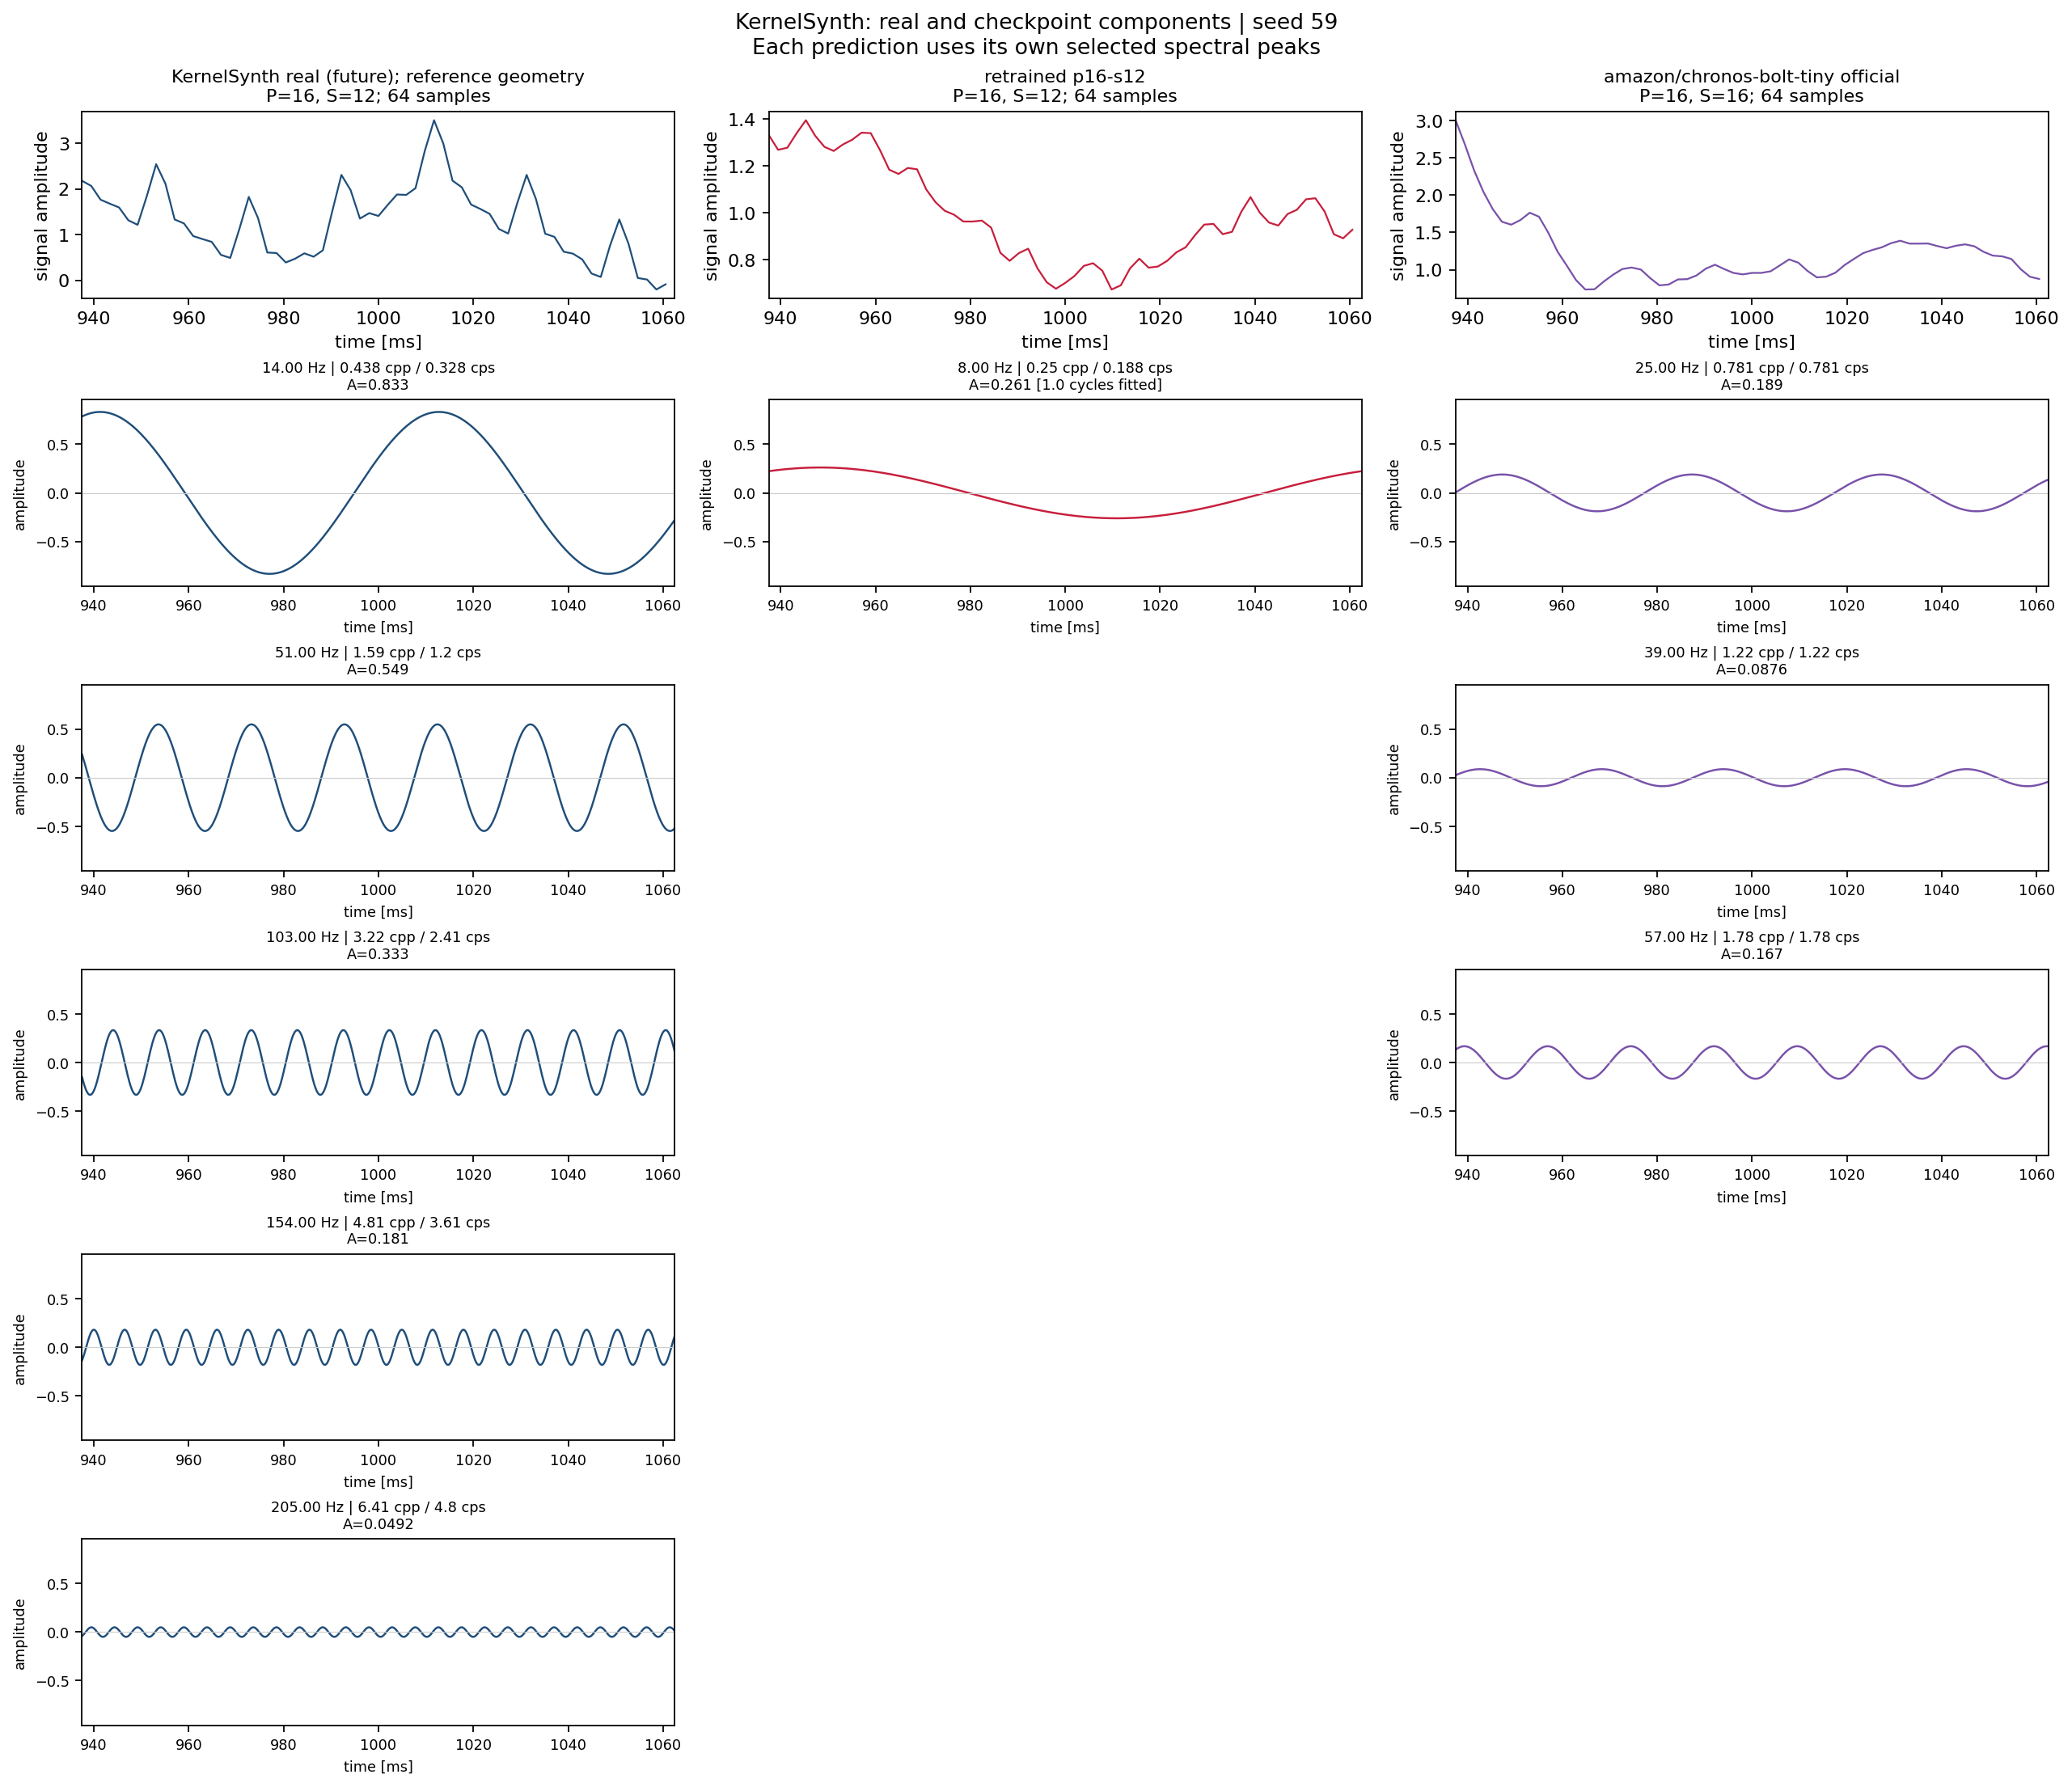
\includegraphics[width=0.97\textwidth,height=0.44\textheight,keepaspectratio]{figures/FIG_E3_kernelsynth_p16-s12_main_components_seed59.png}
    \par\vspace{6pt}
    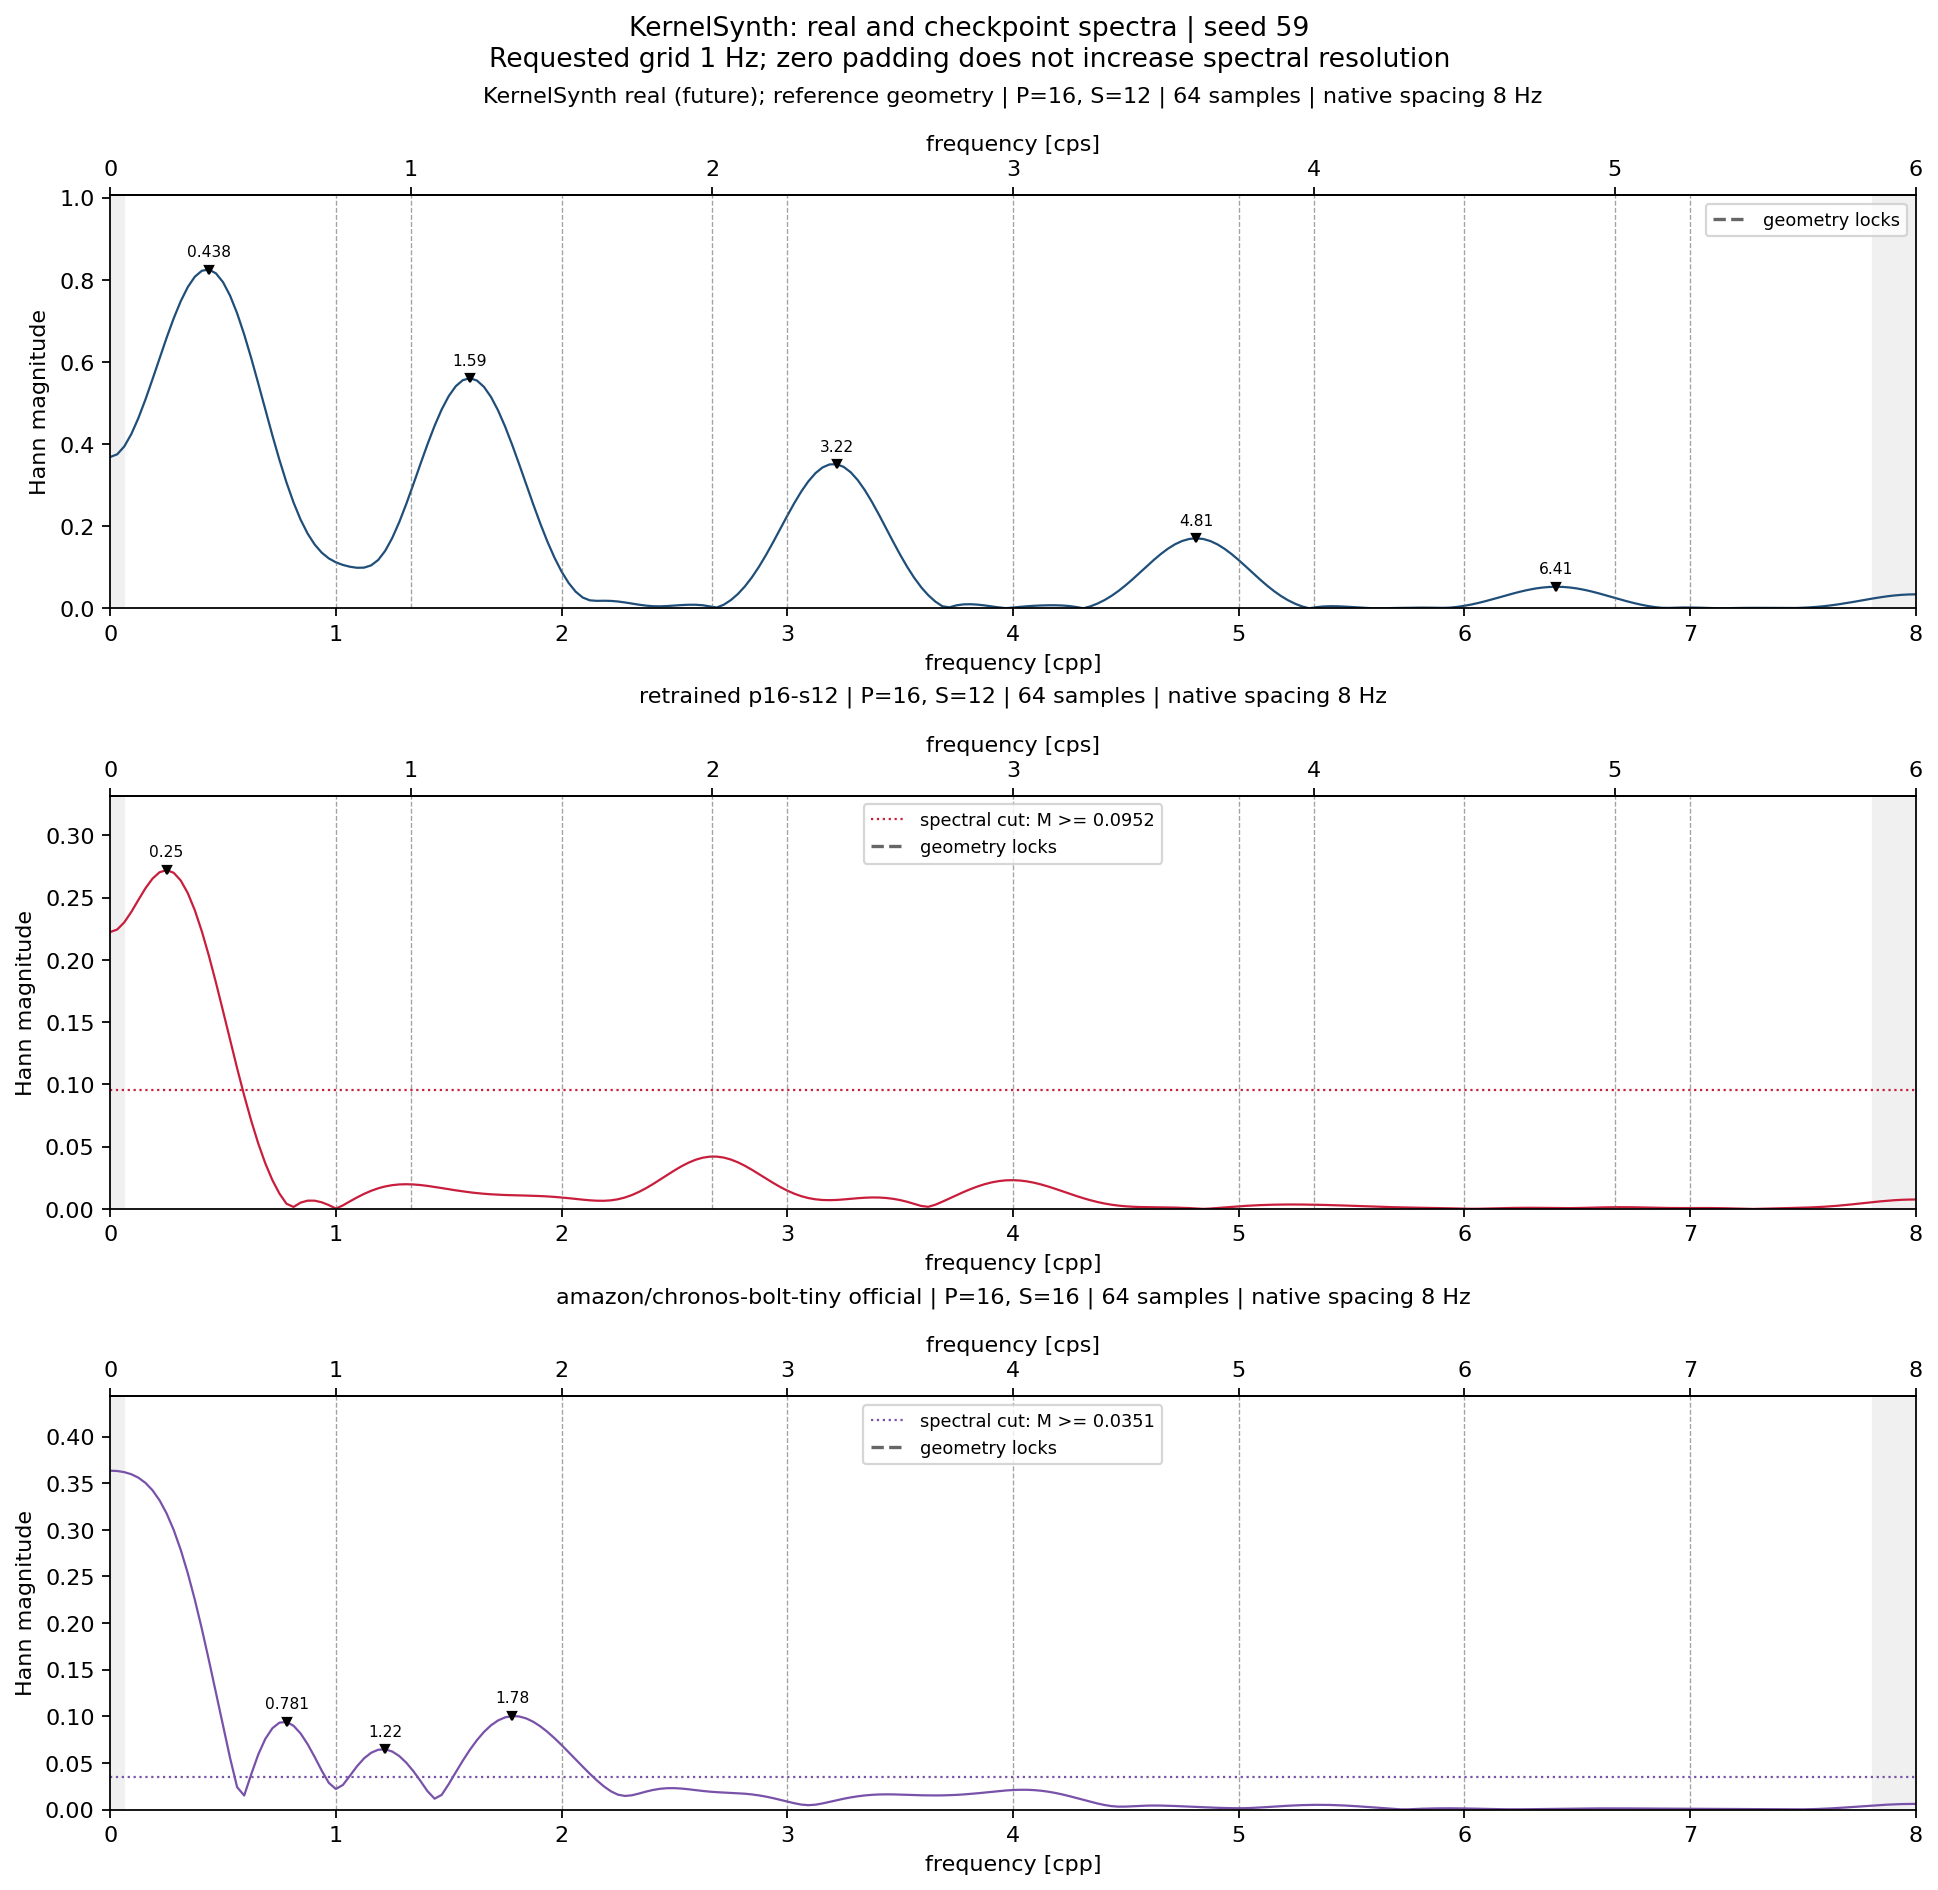
\includegraphics[width=0.97\textwidth,height=0.30\textheight,keepaspectratio]{figures/FIG_E4_kernelsynth_p16-s12_spectra_seed59.png}
\caption{KernelSynth, one draw. Above, the components of the real continuation, of the retrained geometry and of the published checkpoint, each forecast made from the same context; below, the spectra those components were read from. Both sides are estimated, since the generator names no frequencies. \textcolor{red}{\textbf{Placeholder, to be replaced with the $P=S=16$ reference geometry (seed~59 shown here on the retrained p16-s12).} The real continuation carries five lines, from $14$ to $205$\,Hz ($0.44$ to $6.41$ cycles per patch). The retrained model keeps only the slowest content, a single line at $8$\,Hz with about a third of the real amplitude and fitted over one cycle, and returns none of the lines above $50$\,Hz. The published model keeps three weak lines between $25$ and $57$\,Hz beside a strong near-zero component, so it retains more structure than the retrained one, but neither returns the lines at $103$, $154$ and $205$\,Hz.}}
    \label{fig:decompKS}
\end{figure*}

\begin{figure*}[p]
    \centering
    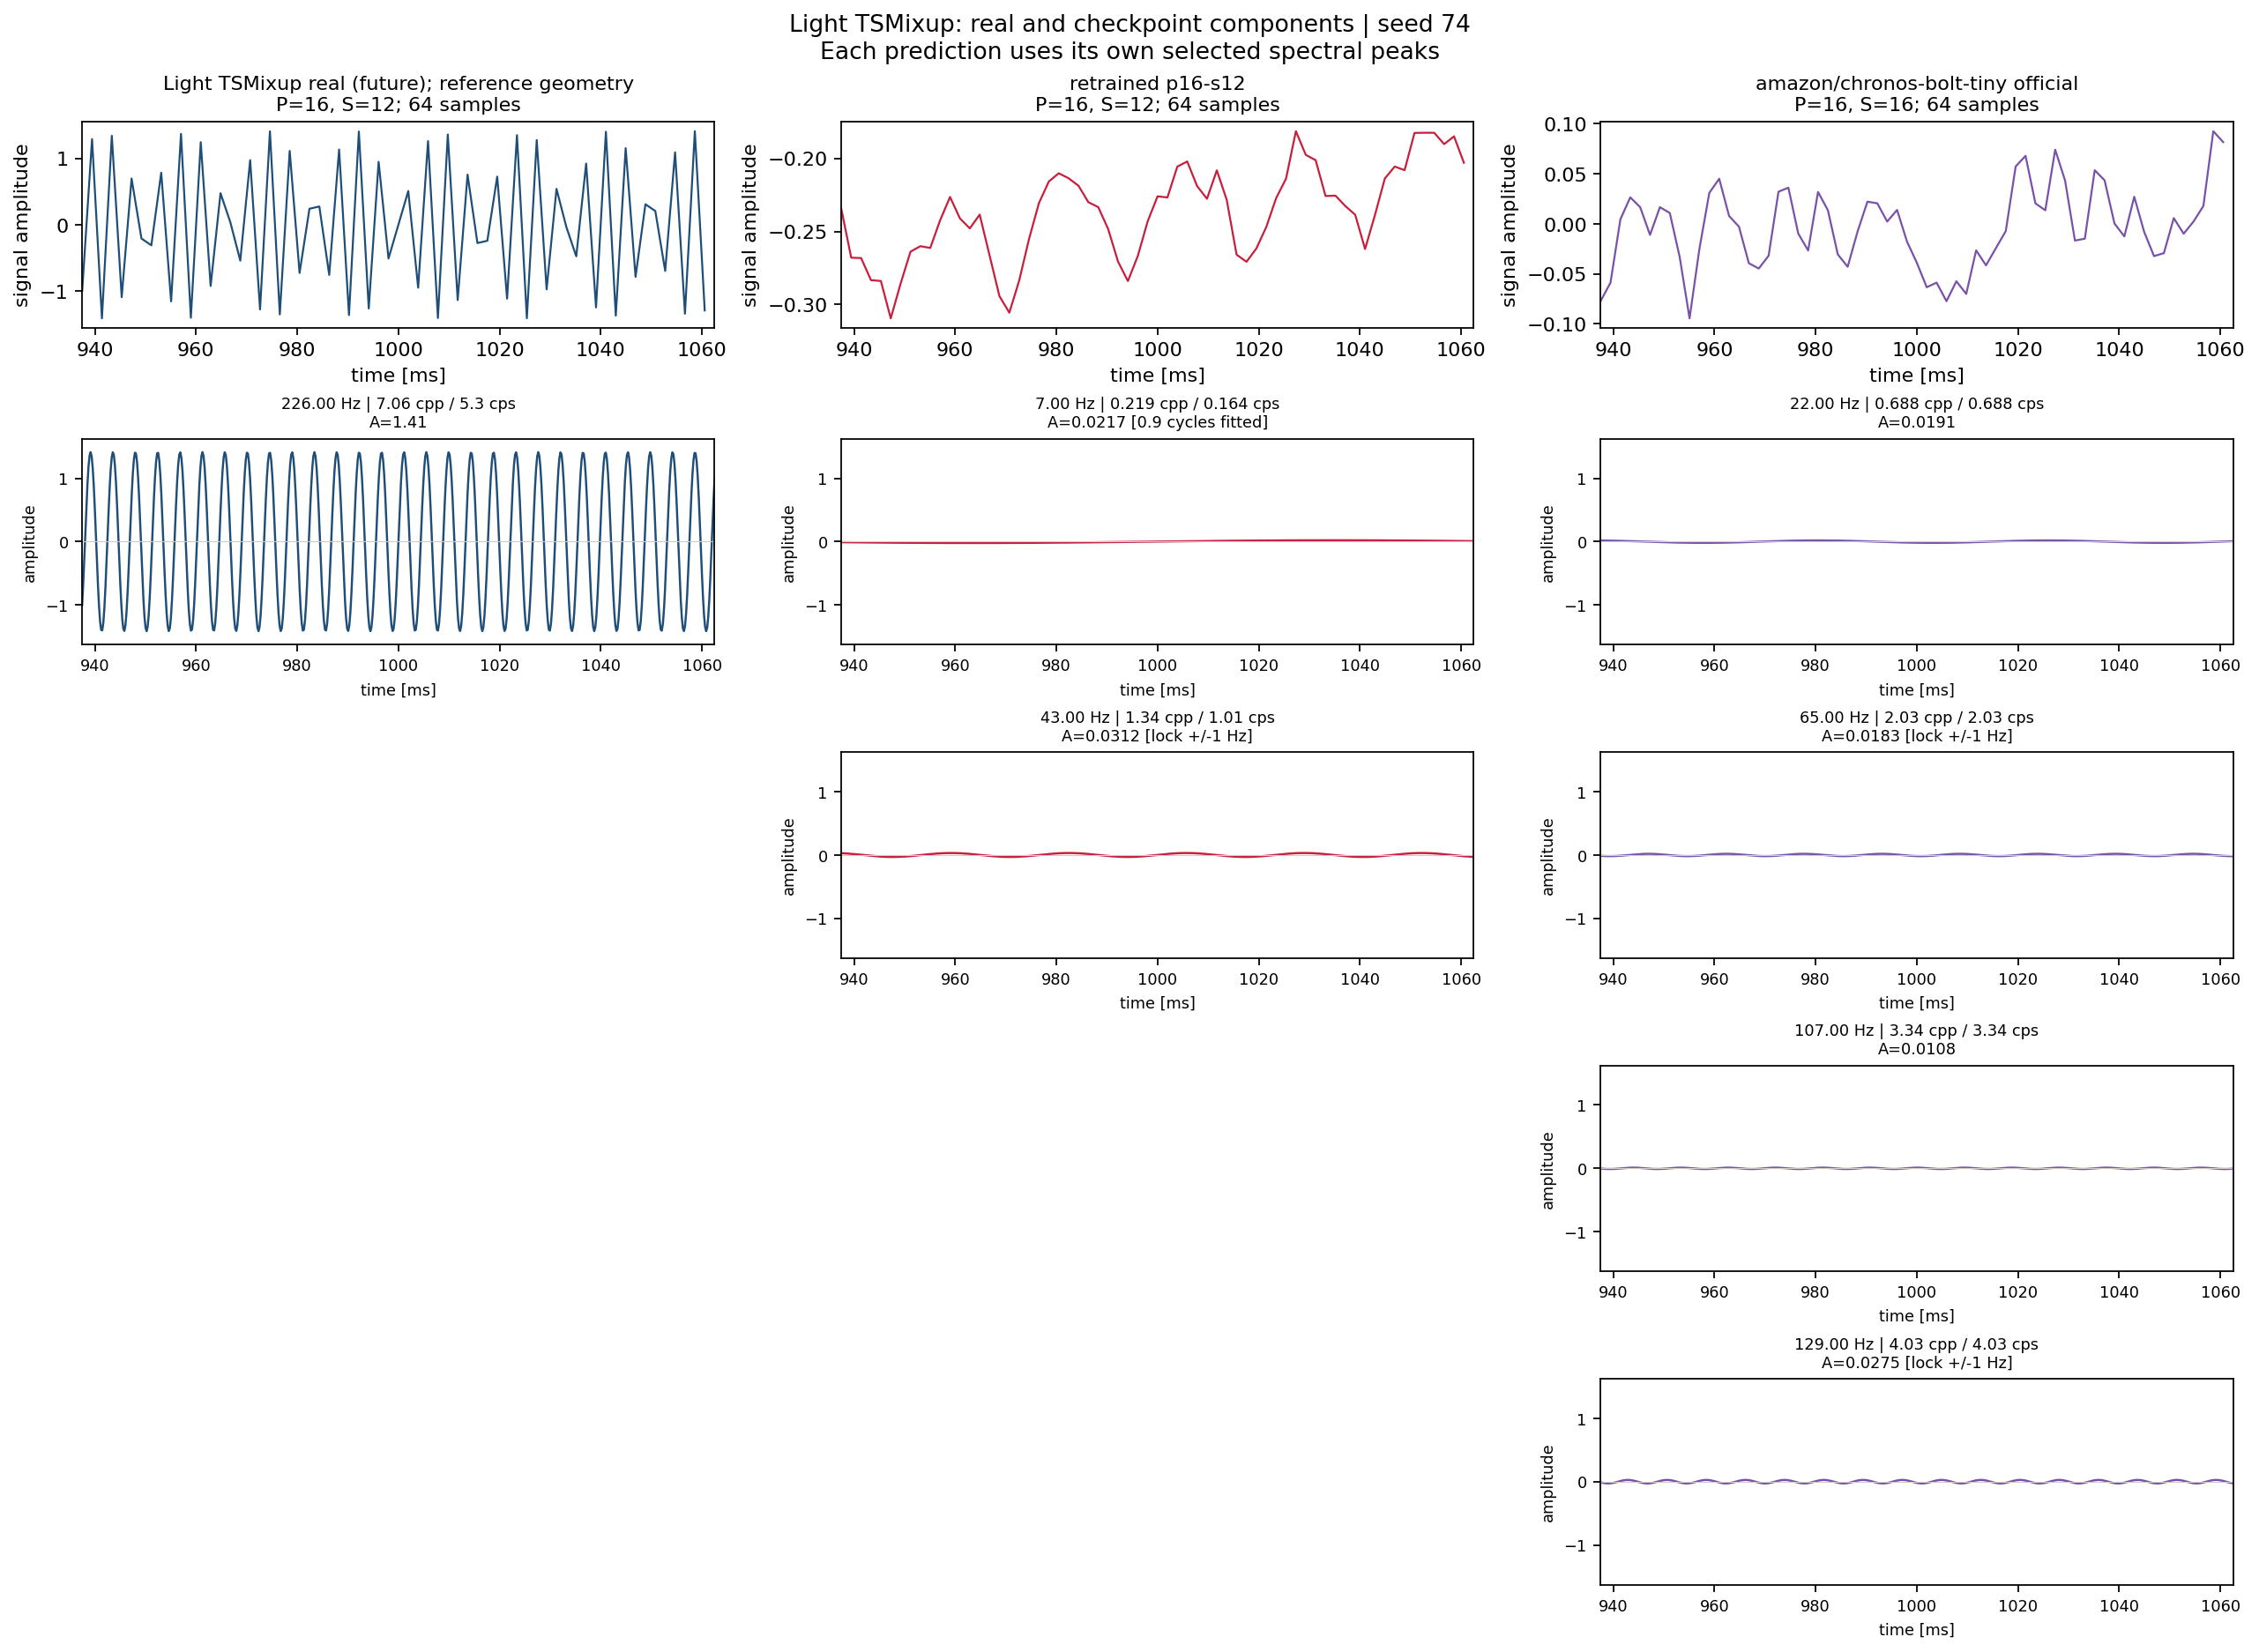
\includegraphics[width=0.97\textwidth,height=0.44\textheight,keepaspectratio]{figures/FIG_E3_tsmixup_p16-s12_main_components_seed74.png}
    \par\vspace{6pt}
    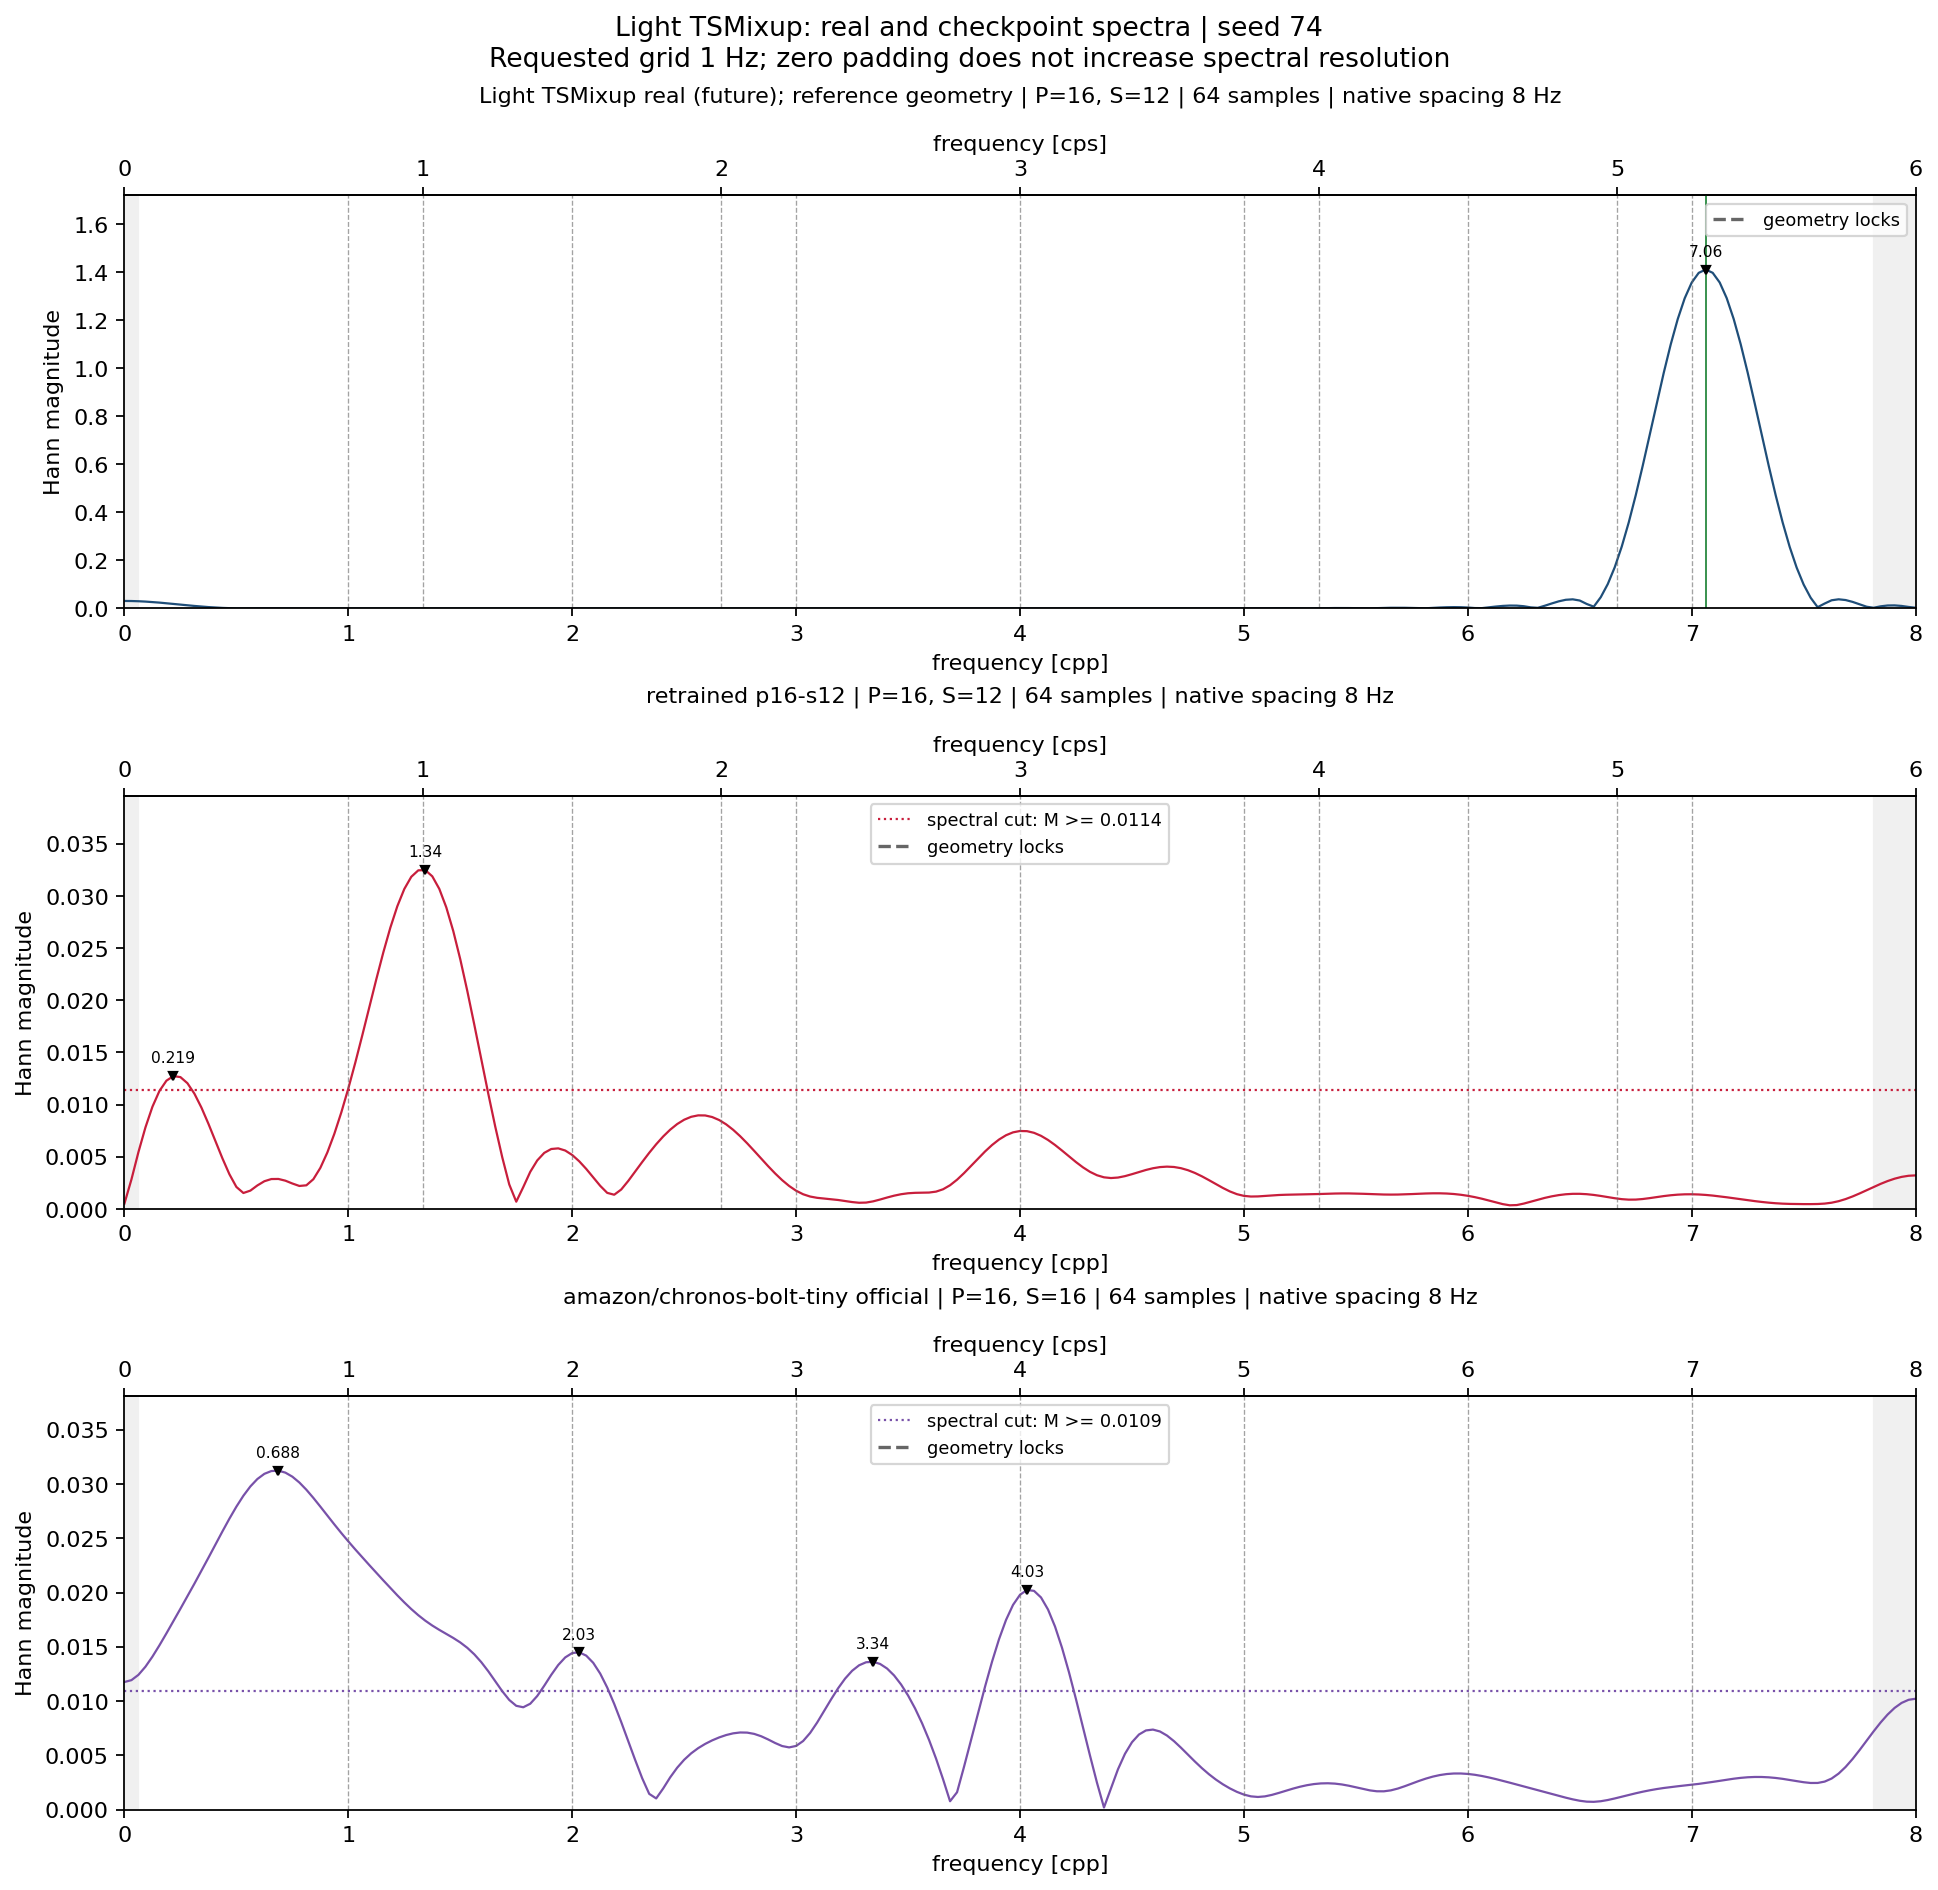
\includegraphics[width=0.97\textwidth,height=0.30\textheight,keepaspectratio]{figures/FIG_E4_tsmixup_p16-s12_spectra_seed74.png}
\caption{Light TSMixup, one draw, read as \autoref{fig:decompKS}. The real side lists the frequencies the generator drew rather than estimating them. \textcolor{red}{\textbf{Placeholder, to be replaced with the $P=S=16$ reference geometry (seed~74 shown here on the retrained p16-s12).} The draw holds a single component at $226$\,Hz ($7.06$ cycles per patch, $2$\,Hz from the patch site at $224$\,Hz) with amplitude $1.41$. Neither checkpoint returns it: both forecasts are nearly flat, with residual lines two orders of magnitude weaker than the input. Several of those residual lines fall within one hertz of the checkpoint's own candidate sites, at $43$\,Hz for the retrained model and at $65$ and $129$\,Hz for the published one, so the forecasts carry content on their combs that the input did not.}}
    \label{fig:decompTS}
\end{figure*}

\subsection{The recovery count}

The single draws show what happens to one realisation; the count behind \autoref{tab:decomposition} asks how often an added component survives. For each generator one hundred backgrounds are drawn with the recipe above and reused unchanged for every checkpoint. Each geometry then receives one hundred paired trials: in the lock trial a tone is added at one of that geometry's candidate sites, the sites being cycled so that each is used about equally often, and since no geometry has a hundred sites in band, sites recur. In the control trial the same background receives a tone at a nearby frequency, placed below or above the site in equal proportion and more than $2$\,Hz from every candidate of that geometry. The tone has an amplitude of one and a half times the background standard deviation and the same phase in both trials of a pair, and the sum is not renormalised afterwards. The published checkpoint and the retrained $P=S=16$ share the same candidate sites and receive exactly the same signals.

Each forecast is decomposed as above, with up to eight candidate lines and the $35\%$ cut. A trial counts as recovered when any retained line lies within $\pm1$\,Hz of the added tone, bounds included. All one hundred trials remain in each denominator, and a forecast that cannot be produced stops the count rather than being dropped from it, so a geometry cannot improve its rate by failing on the difficult cases.

Three limits bound what the count can say, the first being that it measures presence in the output and not attribution, since the background may already carry energy near the added frequency and nothing is subtracted for it. The one-hertz tolerance is finer than the native spacing, so a recovered line is one located near the tone, not one resolved from its neighbours. And the count carries no interval, so it describes the geometries at a high level and is not a statistical test.
